% БҮЛЭГ 4 — ӨГӨГДЛИЙН БОЛОВСРУУЛАЛТ
% Эх: diploma_0.2v.docx, БҮЛЭГ 4. ӨГӨГДЛИЙН БЭЛТГЭЛ

\chapter{Өгөгдлийн боловсруулалт}
\label{Chapter4}

%-------------------------------------------------------------------------------
\section{Өгөгдлийн цуглуулалт}

Системийн сургалтын болон туршилтын өгөгдлийн багц нь хоёр үндсэн эх
сурвалжаас бүрдэнэ: news.mn мэдээний сайтын сэтгэгдлийн хэсэг болон
Facebook-ийн нийтийн хуудас, бүлгүүд (groups). Эх сурвалж бүрийг сонгосон
үндэслэл нь домайны олон талт байдлыг (domain diversity) хангах явдал юм ---
зөвхөн нэг платформоос авсан өгөгдөл загварыг тухайн платформын хэлбэр, ярианы
хэв маягт хэт тохируулж болзошгүй.

\textbf{Кирилл бичгийн шүүлтийн шалгуур.} Цуглуулалтын шатанд кирилл
тэмдэгтийн эзлэх хувийг тооцоолох автомат шүүлтийн алхам хэрэгжүүлнэ. Нийт
тэмдэгтийн $85$ хувиас дээш нь кирилл тэмдэгт байхыг шаардлага болгох бөгөөд
энэ босгоос доогуур текстийг датасетад оруулахгүй. Латин үсгийн бичвэр,
монгол-англи холимог (code-switched) текст, болон романчилсан Монгол бичлэг
(жишээлбэл ``bn'', ``yu ve'', ``zgr'') бүгд хасагдана. Энэхүү шийдэл нь
MN-BERT-ийн кирилл корпус дээр суурилсан токенчлолын үр ашгийг бүрэн
хэрэгжүүлэхэд зайлшгүй шаардлагатай.

news.mn эх сурвалж нь нийгэм, улс төр, эдийн засаг, спорт, соёл зэрэг олон
сэдвийн текст агуулдаг бөгөөд харьцангуй урт, бичгийн хэлний шинжтэй
сэтгэгдлүүд давамгайлдаг. Харин Facebook-ийн нийтийн хуудас болон бүлгүүдэд
ярианы хэлний хэлбэр, emoji агуулсан богино сэтгэгдлүүд зонхилох хандлагатай
байдаг тул хэрэглэгчдийн бодит онлайн харилцааны хэлбэрийг илүү сайн тусгаж
өгдөг. Гэсэн хэдий ч энэ платформоос цуглуулсан өгөгдөлд кирилл бичгийн
шүүлтийн алхам онцгой чухал байдаг бөгөөд учир нь латин үсгийн бичлэг болон
code-switching харьцангуй түгээмэл тохиолддог. Ийнхүү хоёр өөр шинж чанартай
эх сурвалжаас цуглуулсан, кирилл шүүлтийг давсан dataset нь загварын хэрэглэгдэх
орчны олон талт байдлыг хангах боломжийг бүрдүүлнэ.

Цуглуулалтын техникийн хувьд: news.mn-ийн хувьд сайтын ачааллыг тооцоолсон
web scraping ашиглана; Facebook-ийн хувьд Graph API-ийн нийтийн мэдээллийн
хандалтын боломжид тулгуурлана. Цуглуулах хугацааны хүрээ нь 2024--2025 он
байх бөгөөд домайны тэнцвэргүй байдлыг (domain bias) бууруулахын тулд сэдэв
болон платформ бүрээс жигд хувь авах stratified sampling арга ашиглана.

%-------------------------------------------------------------------------------
\section{Өгөгдлийн цэвэрлэгээ ба урьдчилсан боловсруулалт}

Цуглуулсан хам текст (raw text) нь олон хэлбэрийн дуу чимээ (noise) агуулдаг
тул системчилсэн цэвэрлэгээний pipeline (preprocessing pipeline) зайлшгүй
шаардлагатай. Боловсруулалтын дараах үе шатуудыг дараалсан байдлаар хэрэгжүүлнэ.

\textbf{Кирилл хүчинтэй байдлын шүүлт (Cyrillic validation filtering).}
Pipeline-ийн эхний алхам болгон кирилл хүчинтэй байдлын шүүлт хэрэгжүүлнэ.
Тус алхам нь Unicode тэмдэгтийн ангиллыг ашиглан кирилл тэмдэгтийн харьцааг
тооцоолно. Нийт утгатай тэмдэгтийн 85 хувиас дээш нь кирилл биш бол тухайн
бичвэрийг хасна. Уг босго нь тоо, цэг таслал зэрэг кирилл бус боловч утгатай
тэмдэгтүүдийг зөвшөөрч, цэвэр латин болон code-switched текстийг хасахаар
тохируулагдана. Энэхүү алхам нь токенчлол болон бусад боловсруулалтын алхамуудын
өмнө явагдах нь чухал, учир нь MN-BERT-ийн vocabulary нь кирилл корпус дээр
суурилсан тул кирилл бус текст токенчлолын чанарыг эрс бууруулна.

\textbf{Текст нормчлол.} HTML тэмдэгт болон URL хаягийг хасна; тусгай тэмдэгт
болон тоог тохирсон нэрлэсэн токенд (placeholder token) хөрвүүлнэ. Emoji-г
талаарх тусгай тайлбар шаардлагатай: судалгааны хамрах хүрээний тодорхойлолтын
дагуу emoji болон мультимедиа элементүүд загварын ангиллын оролтын онцлог шинж
(semantic feature) болгон ашиглагдахгүй. Гэвч emoji-г preprocessing явцад
текстийн бүтцийг хадгалах зорилгоор нэрлэсэн placeholder токенд (жишээлбэл
{[}EMOJI{]}) хөрвүүлнэ --- энэ нь MN-BERT токенчлолын тогтвортой байдлыг
хамгаалах техникийн арга хэмжээ бөгөөд уг токенууд загварын утга-семантик
боловсруулалтад оролцохгүй. Давтагдсан цагаан зай болон шугам завсар зэргийг
мөн арилгана.

\textbf{Токенчлол.} Монгол хэлний agglutinative онцлогт тохируулсан MN-BERT-ийн
SentencePiece tokenizer ашиглана. Энэ tokenizer нь Монгол кирилл корпус дээр
сургагдсан тул кирилл бичгийн нийлмэл нөхцөлт үгийн бүтцийг морфологийн
тогтвортой байдлаар дэд үгийн (subword) түвшинд задалдаг. Кирилл шүүлтийг давсан
өгөгдөл дээр тус tokenizer оновчтой ажиллах тул дээрх шүүлтийн алхам болон энэ
алхам хоорондоо нягт уялдаатай.

\textbf{Стоп үг хасах.} Монгол хэлний тусгайлсан стоп үгсийн жагсаалт
боловсруулна. Ерөнхий стоп үгс (``нь'', ``бол'', ``байна'', ``гэж'') болон
домайнд хамаарах нийтлэг үгсийг хасах бөгөөд хэт их хасалт нь агуулгын ялгалтад
шаардлагатай мэдрэмж бүхий үгийг алдагдуулах тул хасалтын босгыг (threshold)
туршилтаар тогтооно. Стоп үгсийн жагсаалт нь зөвхөн кирилл бичгийн хэлбэрийг
агуулна.

\textbf{Нормчлол ба морфологийн боловсруулалт.} Том, жижиг үсгийн хөрвүүлэлт,
үгийн үндэс олох (stemming) ажиллагааг хэрэгжүүлнэ. Монгол хэлний нийлмэл
дагаварт үгийн бүтцийг зохих ёсоор задлах тусгайлсан арга зүйг туршилтаар
тодорхойлно.

%-------------------------------------------------------------------------------
\section{Annotation --- Шошгологдолтын стратеги}

Өгөгдлийн шошгололт нь дөрвөн ангилалыг хамарна: Positive (эерэг хандлага),
Neutral (саармаг, мэдээллийн), Toxic Negative (хортой, доромжилсон, дарамтлагч),
Constructive Criticism (аргументтай, сайжруулах санал агуулсан сөрөг хандлага).
Шошгологдолтын стандарт нарийн, тодорхой заавар бэлтгэж, нийт 3
тайлбарлагч (annotator) ажилласан.

10,000 сэтгэгдлийг богино хугацаанд чанартай шошголохын тулд бид ``стандарт
шошгоны стратеги''-ийг ашигласан. Монгол хэлний агуулгыг шууд ангилахын оронд
Positive, Neutral, Toxic Negative, Constructive Criticism гэсэн олон улсын
стандарт англи шошгонуудыг ашигласан нь аннотаторуудад объектив хил хязгаарыг
тодорхой хадгалахад тусалж, шошгологдолтын хурд болон тууштай байдлыг эрс
нэмэгдүүлсэн юм. Энэхүү аргачлалын ачаар бакалаврын түвшний судалгаанд
харьцангуй томд тооцогдох 10,000 дээжийг амжилттай бэлтгэж чадсан.

\textbf{Кирилл-онцлогт аннотацийн заавар.} Аннотаторуудад зориулсан гарын авлага
дараах тусгай зааврыг агуулна. Нэгдүгээрт, аннотацид оруулах зөвхөн кирилл
бичгийн текстийг л авч үзнэ --- латин тэмдэгт давамгайлсан, code-switched, эсвэл
романчилсан бичлэг бүхий жишээ аннотацид оруулахгүй бөгөөд эдгээр нь
preprocessing шатанд аль хэдийн хасагдсан байна. Хоёрдугаарт, кирилл бичиглэлтэй
ч агуулгын утга нь тодорхойгүй бол тухайн жишээг ``дүйцэшгүй'' (ambiguous)
хэмээн тэмдэглэж annotation-оос хасна. Гуравдугаарт, Монгол хэлний ирони болон
нутгийн хэлний кирилл хэллэгийг зөв тайлбарлах тусгай жишээ тохиолдлуудыг
гарын авлагад оруулна --- тухайлбал, ``муу'' гэсэн үг сайшаалыг илэрхийлж болох
тул контекстийн дагуу шошгологдолт хийх шаардлага байна.

Аннотаторуудын хоорондын нийцлийг хэмжихэд Cohen's Kappa коэффициент ашиглана.
$\kappa = 0.72$ гарсан нь хангалттай нийцлийг илтгэх бөгөөд зөрөлдсөн тохиолдлуудыг
хэлэлцэж, консенсусын дүгнэлт гаргасан.
 Шошгологдолтын дараа ангиллуудын тоон
тэнцвэрийг шалгаж, мэдэгдэхүйц тэнцвэргүй байдал илэрвэл SMOTE болон
class-weighted арга хэрэглэнэ.

%-------------------------------------------------------------------------------
\section{Өгөгдлийн хайгуулын шинжилгээ (EDA)}

Загвар сургалтын өмнө цуглуулсан 10,000 дээж бүхий өгөгдлийн багцад хайгуулын
шинжилгээ (Exploratory Data Analysis - EDA) хийж, өгөгдлийн бүтэц, онцлог шинжийг
тодорхойлов. Энэхүү алхам нь загварын сургалтын үр дүн болон гарч болох алдааг
урьдчилан таамаглахад чухал ач холбогдолтой.

\textbf{Ангиллын тархалт.} Зураг \ref{fig:label-dist}-т харуулсанчлан датасетад
Constructive Criticism (43.9\%) болон Neutral (30.0\%) ангиллууд давамгайлж байна.
Харин Positive (6.7\%) ангилал хамгийн бага хувийг эзэлж байгаа нь Монгол хэлний
сошиал медиа орчинд сэтгэл хөдлөлийн эерэг өнгө аяс харьцангуй бага, эсвэл
хүмүүс сэтгэл ханамжаа илэрхийлэхээс илүүтэй шүүмжлэх, асуудал хөндөх хандлагатай
байдагтай холбоотой байж болох юм.

\begin{figure}[H]
    \centering
    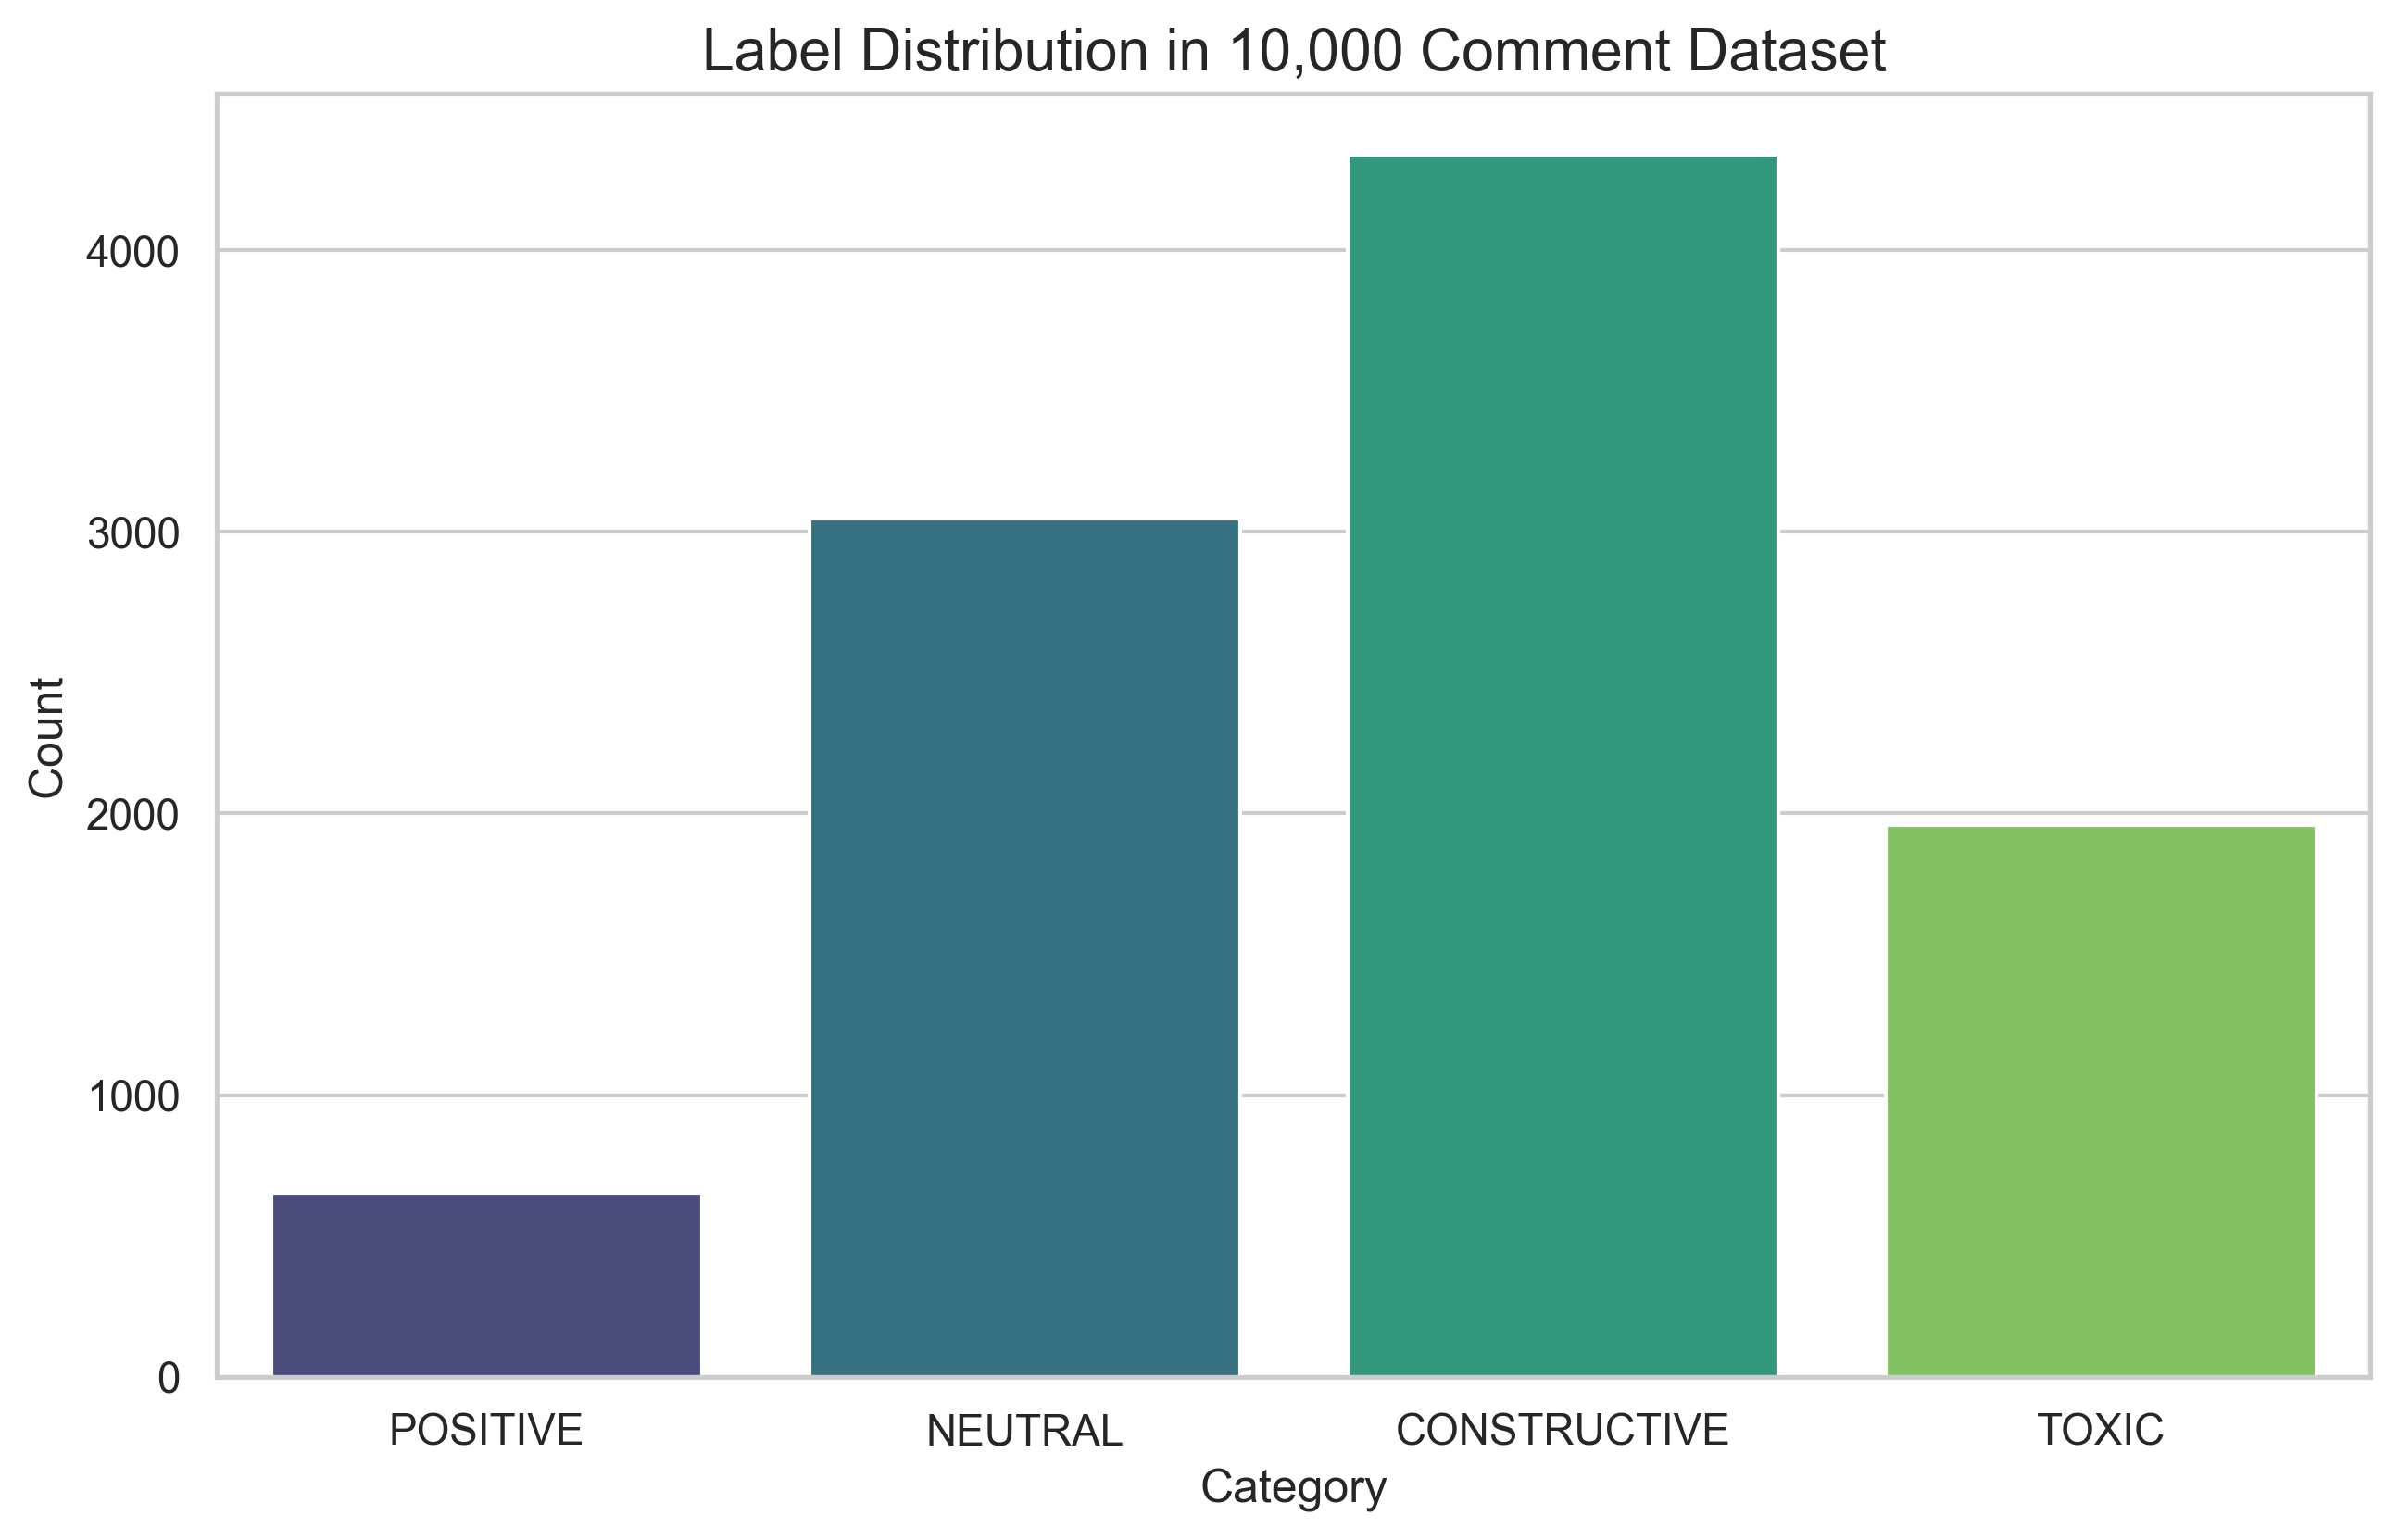
\includegraphics[width=0.8\textwidth]{Figures/EDA/label_distribution.png}
    \caption{10,000 сэтгэгдлийн ангиллын тархалт}
    \label{fig:label-dist}
\end{figure}

\textbf{Сэтгэгдлийн уртын шинжилгээ.} Сэтгэгдлийн уртыг тэмдэгтийн тоогоор
хэмжиж, ангилал тус бүрээр харьцуулав (Зураг \ref{fig:len-dist}). Constructive
Criticism ангиллын сэтгэгдлүүд дунджаар хамгийн урт (median $\approx 150$ тэмдэгт)
байгаа нь шүүмжлэл илэрхийлэхдээ аргумент, тайлбар ашигладаг болохыг харуулж
байна. Нөгөө талаас, Toxic болон Neutral сэтгэгдлүүд харьцангуй богино
байх хандлагатай байна.

\begin{figure}[H]
    \centering
    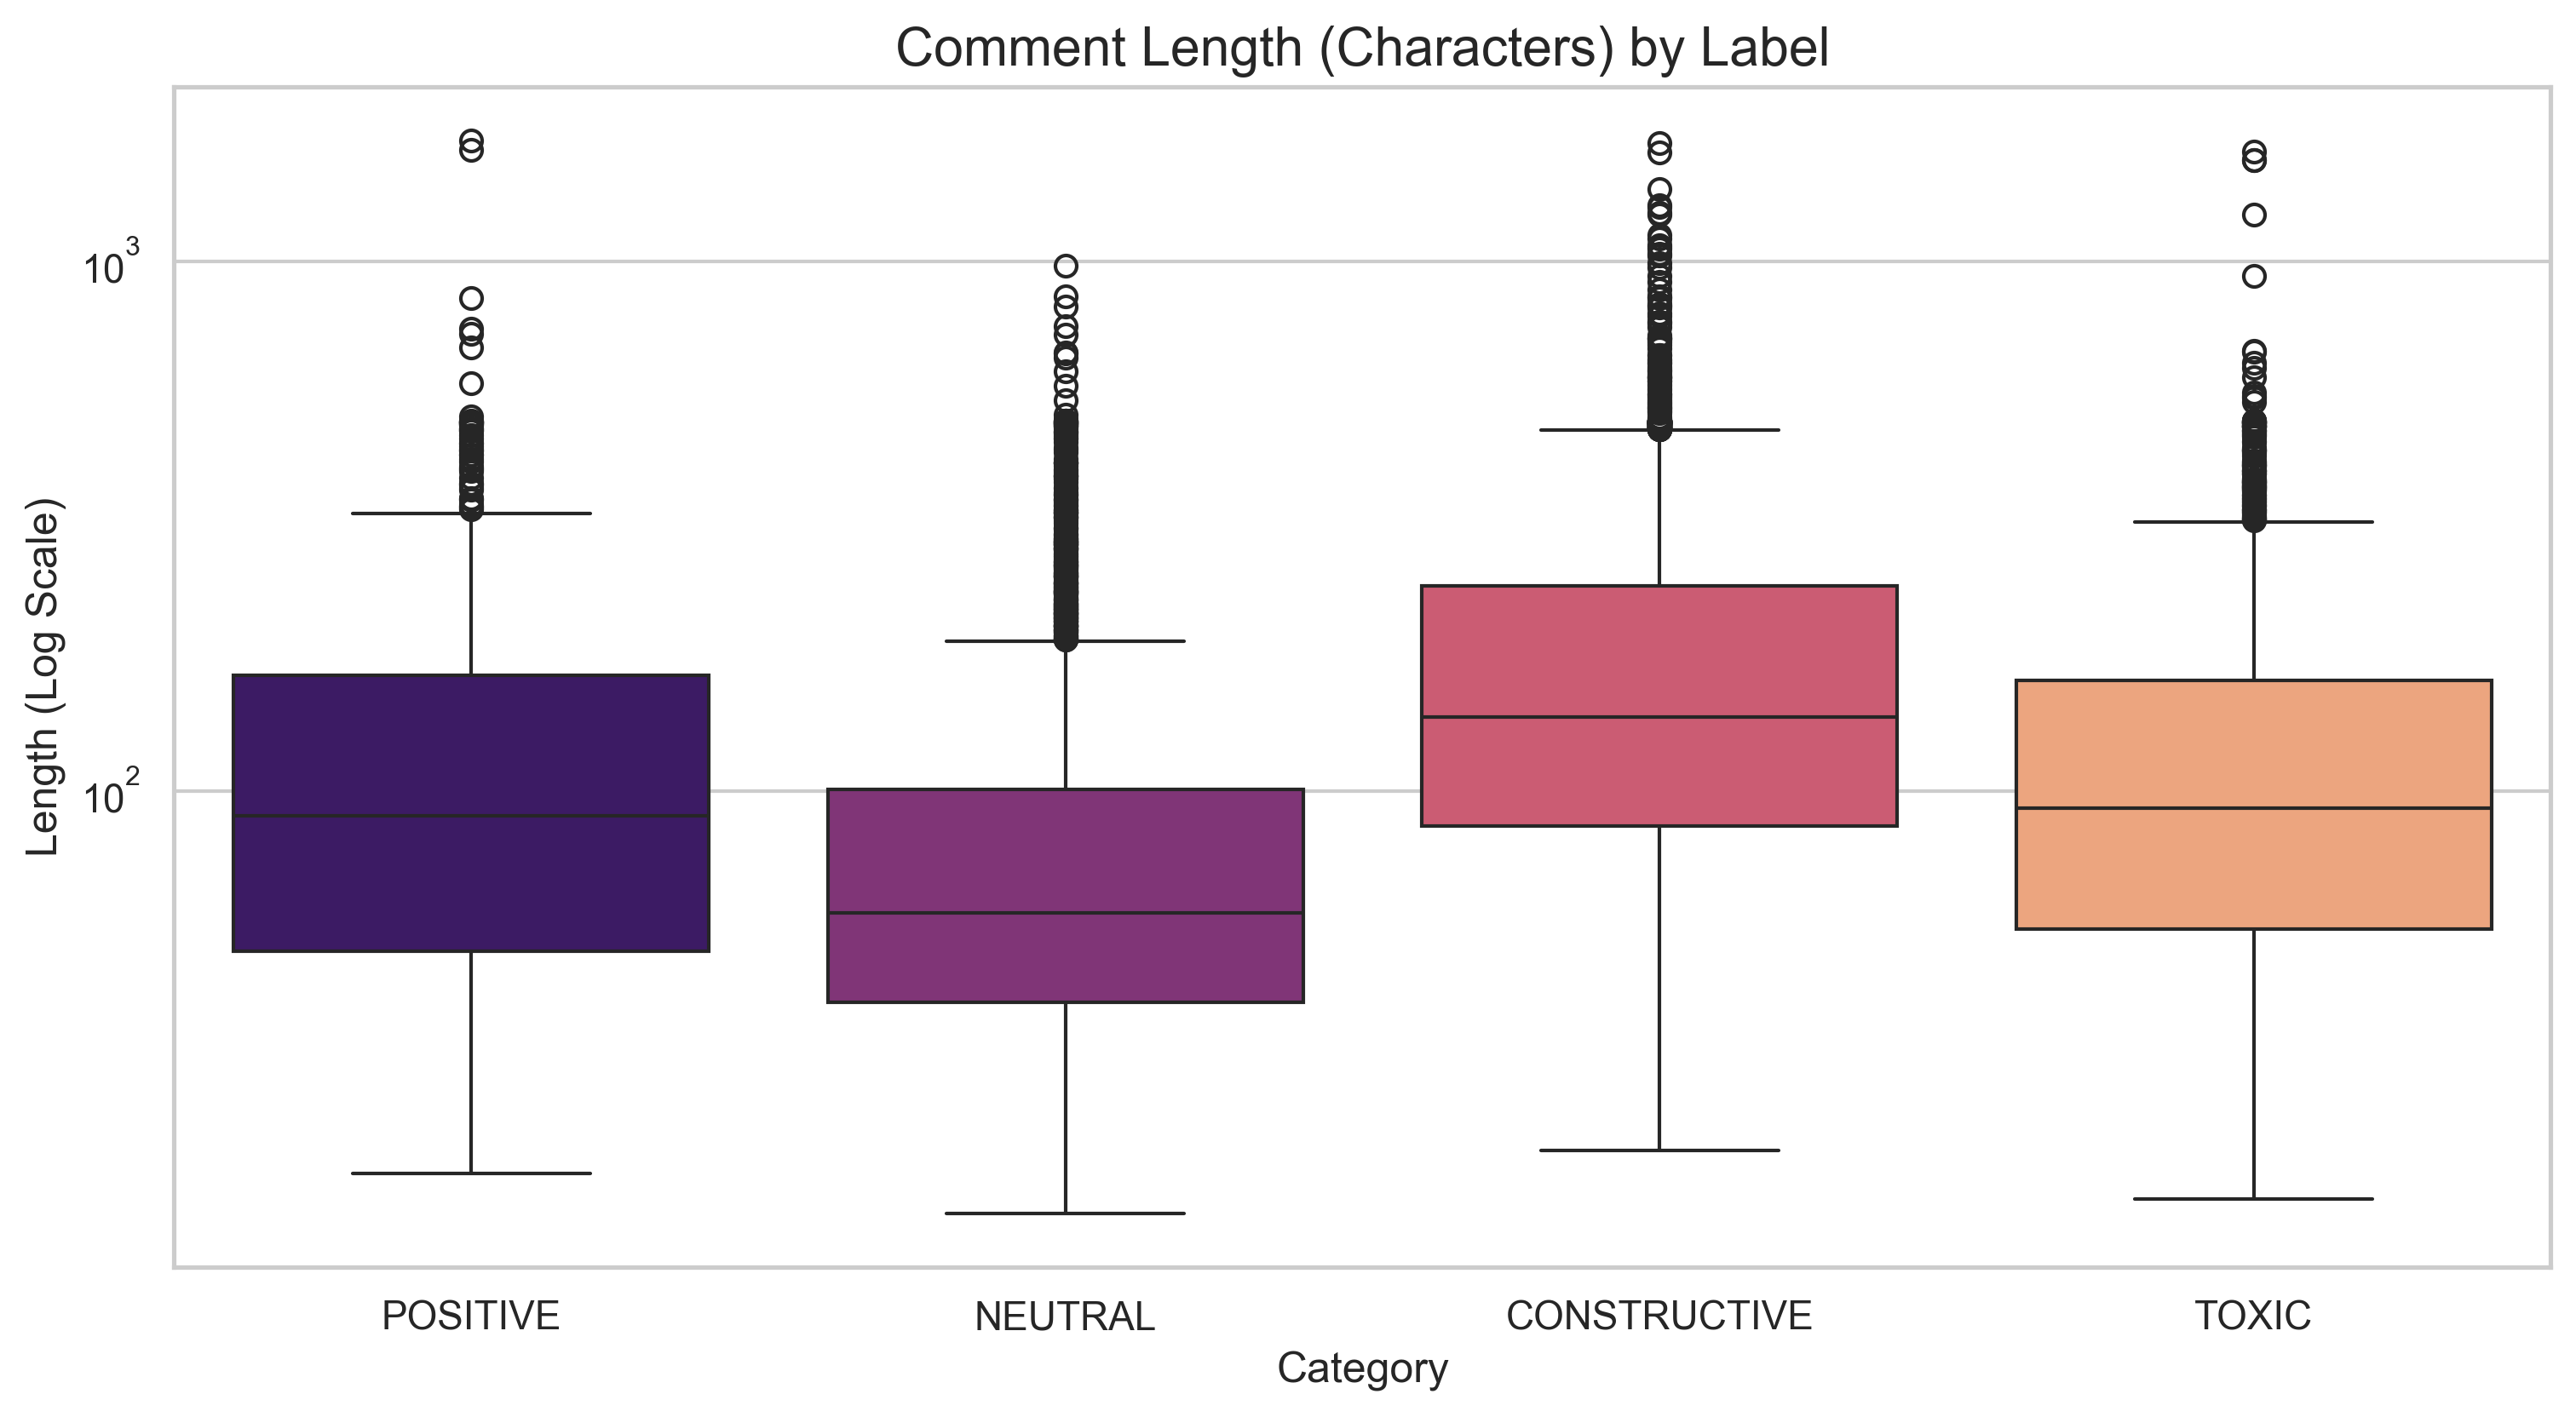
\includegraphics[width=0.8\textwidth]{Figures/EDA/length_distribution.png}
    \caption{Ангилал тус бүрийн сэтгэгдлийн уртын тархалт (Логарифм хэмжээс)}
    \label{fig:len-dist}
\end{figure}

\textbf{N-gram давтамжийн шинжилгээ.} Хортой (Toxic) болон Бүтээлч (Constructive)
ангиллын үгсийн санг ялгахын тулд хамгийн их давтагдсан нэгт үгс (unigrams) болон
хоёртын үгс (bigrams)-ийг шинжлэв. Toxic ангилалд хувь хүн рүү чиглэсэн
доромжлол, хараалын үгс давамгайлж байгаа бол, Constructive ангилалд ``хэрэгтэй'',
``засах'', ``ажлаа хий'', ``болохгүй байна'' гэх мэт асуудал шийдвэрлэх, үр дүн
шаардсан үг хэллэгүүд түгээмэл байна. Энэхүү семантик ялгаа нь бидний дэвшүүлсэн
хоёр шатлалт ангиллын системийн үндсэн логик болох юм.

\begin{figure}[H]
    \centering
    \begin{minipage}{0.48\textwidth}
        \centering
        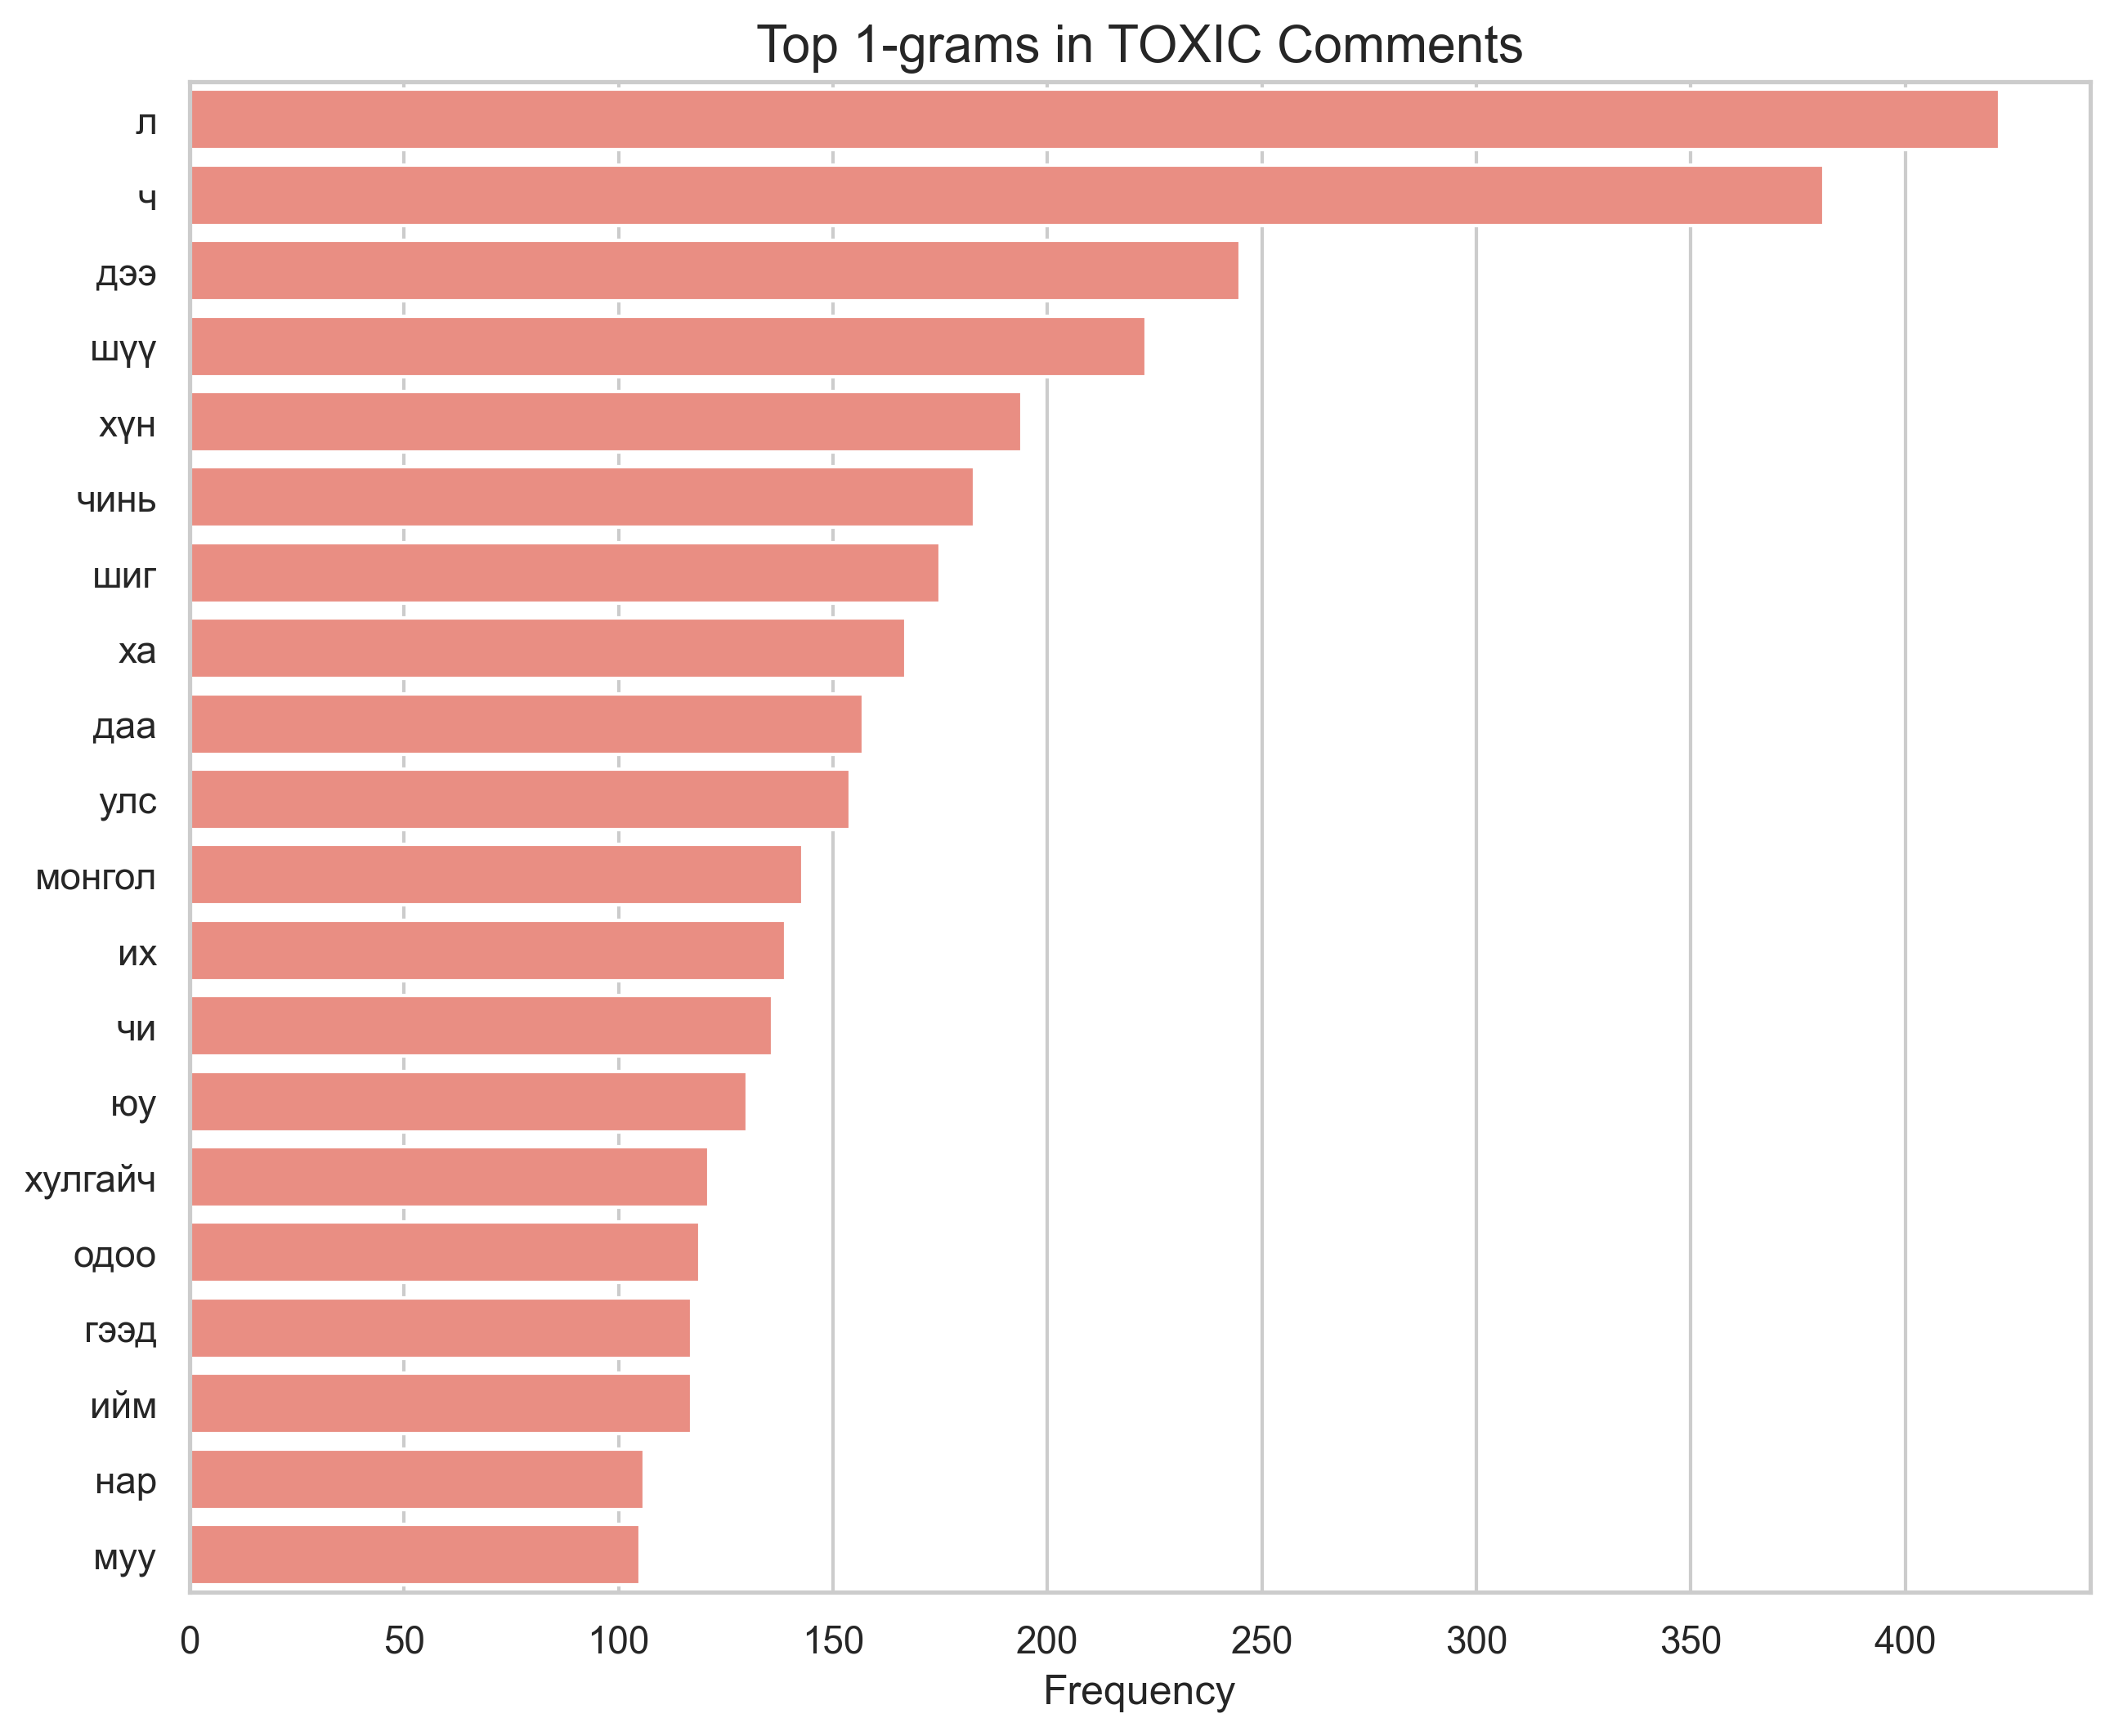
\includegraphics[width=\textwidth]{Figures/EDA/top_1gram_toxic.png}
        \caption{Toxic-unigrams}
    \end{minipage}
    \hfill
    \begin{minipage}{0.48\textwidth}
        \centering
        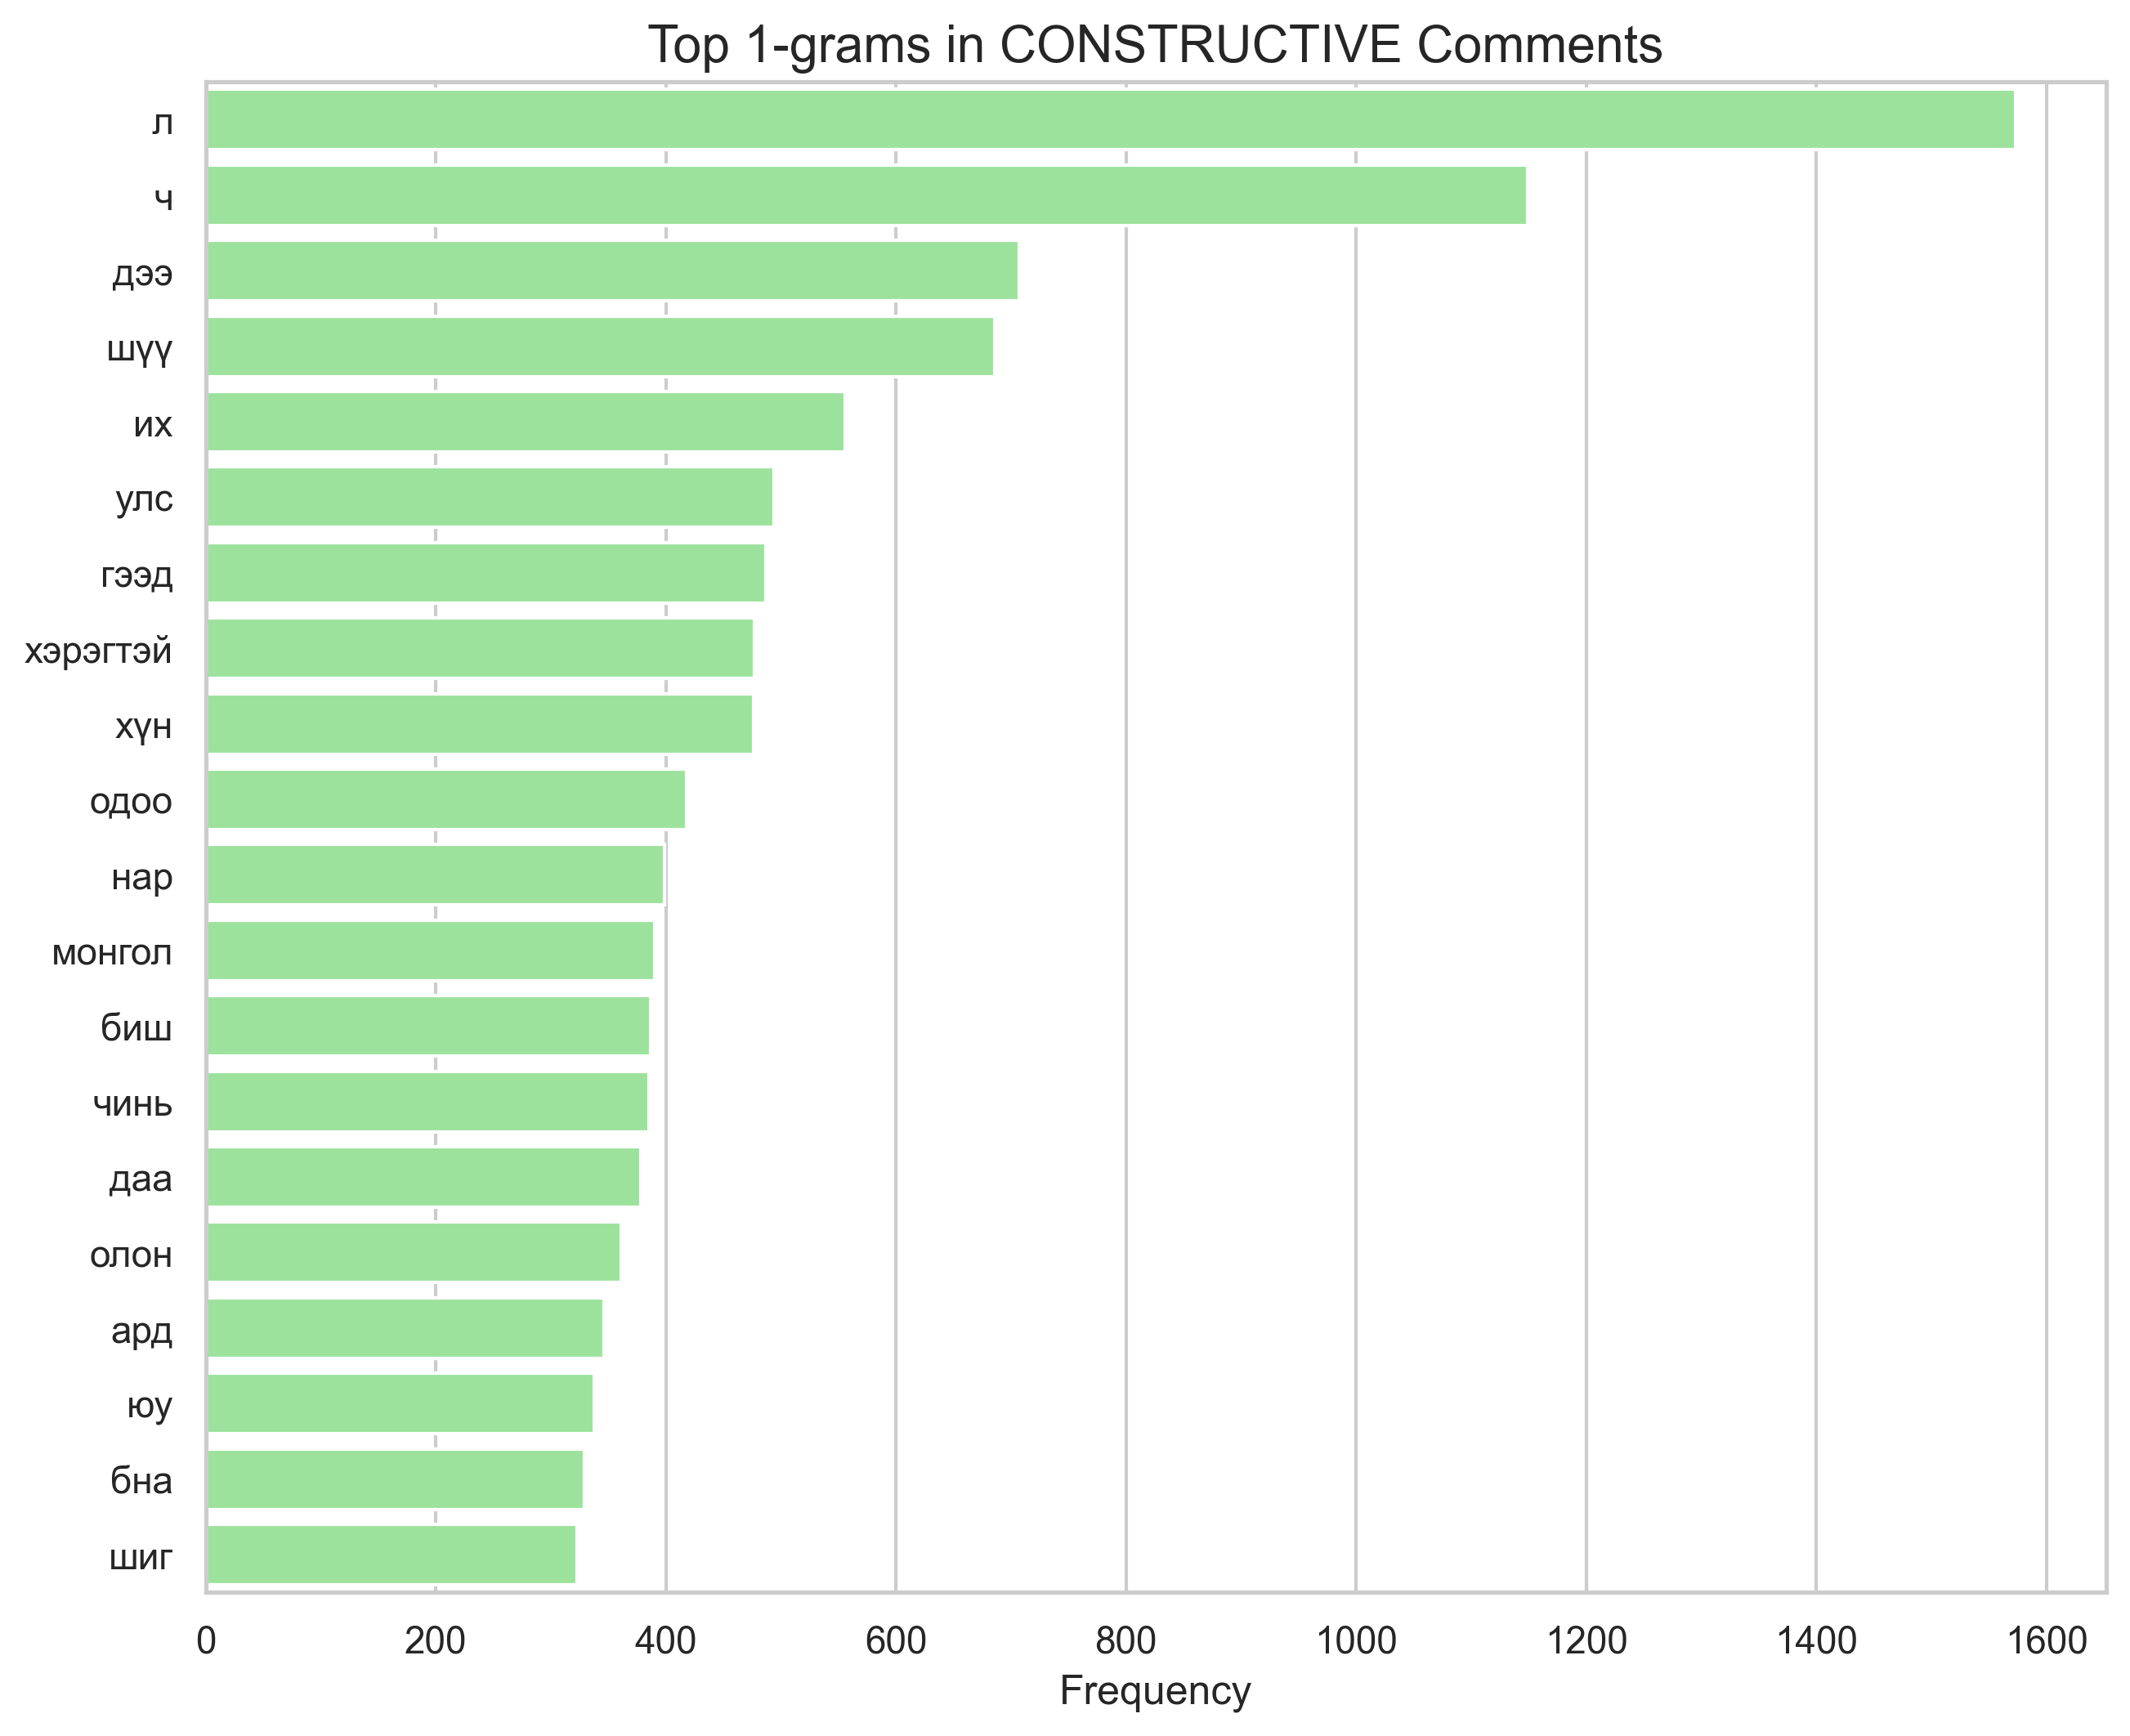
\includegraphics[width=\textwidth]{Figures/EDA/top_1gram_constructive.png}
        \caption{Constructive-unigrams}
    \end{minipage}
\end{figure}

%-------------------------------------------------------------------------------
\section{Dataset хуваалт}

Цуглуулсан болон шошгологдсон dataset-ийг загварыг сургах, тохируулах, туршихад
ашиглах гурван хэсэгт хуваана: сургалтын (training) $70\%$, хэт тохируулгын
(validation) $15\%$, туршилтын (test) $15\%$. Хуваалт нь stratified байх ---
өөрөөр хэлбэл дөрвөн ангилал бүрийн харьцаа хэсэг бүрд тэнцүү хуваарилагдана.
Энэ арга нь тэнцвэргүй ангиллын нөхцөлд загварын дутуу тохируулгын
(underfitting) болон хэт тохируулгын (overfitting) эрсдлийг бууруулдаг.
Туршилтын хэсэг нь загварын сургалтын явцад огт ашиглагдалгүй, зөвхөн эцсийн
гүйцэтгэлийн үнэлгээнд нэг удаа ашиглагдана.

\begin{table}[H]
\centering
\caption{Dataset-ийн ангилал бүрийн жишээний тоо (10,000 дээж)}
\label{tab:data-stats}
\begin{tabular}{@{}lcccc@{}}
\toprule
\textbf{Ангилал} & \textbf{Train (70\%)} & \textbf{Val (15\%)} & \textbf{Test (15\%)} & \textbf{Нийт} \\
\midrule
Positive     & $475$  & $99$  & $100$  & $674$ \\
Neutral      & $2,109$ & $443$ & $443$ & $2,995$ \\
Toxic        & $1,369$ & $287$ & $288$ & $1,944$ \\
Constructive & $3,090$ & $648$ & $649$ & $4,387$ \\
\midrule
\textbf{Нийт} & $\mathbf{7,043}$ & $\mathbf{1,427}$ & $\mathbf{1,530}$ & $\mathbf{10,000}$ \\
\bottomrule
\end{tabular}
\end{table}

%-------------------------------------------------------------------------------
\section{Монгол хэлний онцгой бэрхшээлүүд}

Монгол хэлний NLP-д нийтлэг тулгардаг хэд хэдэн тусгай бэрхшээл байна.
Нэгдүгээрт, agglutinative бүтэц: нэг үгийн үндэст олон дагавар нэмэгдэж, лексик
хэмжигдэхүүн (vocabulary size) огцом нэмэгдэнэ --- энэ нь BoW, TF-IDF зэрэг
арга зүйн гүйцэтгэлийг бууруулдаг. Хоёрдугаарт, бага хэмжээний нийтэд нээлттэй
corpus: Монгол хэлний NLP-д ашиглах том хэмжээний шошгологдсон өгөгдөл туйлын
хомс байгаа нь загварыг сургах, туршихад хүндрэл учруулдаг. Гуравдугаарт,
ярианы болон бичгийн хэлний ялгаа: нийгмийн сүлжээнд ашиглагдах ярианы хэл нь
стандарт бичгийн Монгол хэлнээс ялгаатай болон тогтворгүй байдаг. Дөрөвдүгээрт,
annotation-ийн нийтлэг стандарт байхгүй: Монгол хэлний хортой агуулгын
шошгологдолтын нийтлэг стандарт, corpus байхгүй тул тайлбарлагчдын хоорондын
нийцлийг хангах нь хүнд байдаг.

\textbf{Кирилл-онцлогт хязгаарлалт.} Энэхүү судалгааны датасет болон загвар нь
зөвхөн кирилл бичгийн Монгол хэлний текстэд хамаарна. Латин үсгийн бичвэр,
монгол-англи холимог (code-switched) текст, романчилсан Монгол бичлэг (``bn'',
``yu ve'', ``zgr'' гэх мэт хэлбэр), болон кирилл бус бусад бичиглэлийн хэлбэрүүд
одоогийн системийн хамрах хүрээнд ороогүй. Цахим орчинд code-switching нэлээд
тархсан байдаг тул уг хязгаарлалт нь загварын бодит орчин дахь хэрэглээний
хүрээг зарим хэмжээгээр бууруулж болзошгүй. Гэхдээ энэхүү шийдэл нь MN-BERT-ийн
кирилл корпус дээр суурилсан токенчлолын морфологийн тогтвортой байдлыг
хамгаалж, аннотацийн стандартыг нэгтгэхэд шаардлагатай үндэслэлтэй алхам юм.
Латин бичгийн болон code-switched текстийг дэмжих боломжийг ирээдүйн судалгааны
чиглэл болгон тодорхойлно.

%-------------------------------------------------------------------------------
\section{Бүлгийн дүгнэлт}

Өгөгдлийн бэлтгэлийн бүлэгт цуглуулалтын эх сурвалж, цэвэрлэгээний pipeline,
шошгологдолтын стратеги, dataset хуваалт болон Монгол хэлний тусгай бэрхшээлийг
тодорхойлсон. Систем зохион байгуулалтын чанар нь эцэст нь сургалтын өгөгдлийн
чанараас шалтгаалдаг учраас өгөгдлийн бэлтгэлийн энэ бүлэг нь бүхэл ажлын
чухал суурь болдог. Дараагийн бүлэгт системийн архитектур болон загварын зохион
байгуулалтыг нарийвчлан тайлбарлана.
